 \documentclass[a4paper,12pt]{article} 
\usepackage[T2A]{fontenc}			
\usepackage[utf8]{inputenc}			
\usepackage[english,russian]{babel}	
\usepackage{amsmath,amsfonts,amssymb,amsthm,mathrsfs,mathtools} 
\usepackage[colorlinks, linkcolor = purple, citecolor = purple]{hyperref}
\usepackage{xcolor}
\usepackage{xpatch}
\usepackage{marvosym}
\usepackage{cancel}
\usepackage{floatrow}
\usepackage{commath}
\usepackage{upgreek}
\usepackage{lipsum}
\usepackage{mhchem}
\usepackage{chemfig}
\usepackage{multirow}
\usepackage{tikz}
\usepackage{titletoc}
\usepackage{pgfplots}
\usepackage{wrapfig}
\usepackage{chngcntr}
\usepackage{makecell}
\usepackage{stackengine,graphicx}
\usepackage{cmap}
\usepackage{indentfirst}
\usepackage{tocloft}
\usepackage{setspace}
\usepackage{titlesec}
\usepackage{soul}
\usepackage[stable]{footmisc}
\usepackage{tocloft}
\usetikzlibrary{positioning}
\usepackage{caption}
\usepackage{subfig}
\pgfplotsset{width=10cm,compat=1.9}
\tikzset{>=stealth}
\usepackage[left=2cm,right=2cm,top=2cm,bottom=3cm,bindingoffset=0cm]{geometry}
%\DeclareMathOperator*{\esssup}{ess\,sup}
\DeclareMathOperator*{\tr}{tr}
\DeclareMathOperator*{\Ker}{Ker}
\DeclareMathOperator*{\Rea}{Re}
\DeclareMathOperator*{\Ima}{Im}
\DeclareFontEncoding{LS2}{}{\noaccents@}
\DeclareFontSubstitution{LS2}{stix}{m}{n}
\DeclareSymbolFont{arrows3}{LS2}{stixtt}{m}{n}
\DeclareMathSymbol{\squareulblack}{\mathord}{arrows3}{"88}
\date{\vspace{-10pt}}
\author{Дорогинин Д.В. Б02-825бф\\
Матвеев Г.А. Б02-824бф}
\title{\textbf{Электронный парамагнитный резонанс.}}


\theoremstyle{definition}
\newtheorem*{definition}{Определение}
\newtheorem{statement}{Предложение}
\newtheorem{lemma}{Лемма}
\newtheorem{theorem}{Теорема}
\newtheorem*{theorem*}{Теорема}
\newtheorem*{corollary}{Следствие}
\newtheorem*{example}{Пример}
\setcounter{tocdepth}{2}
%\renewcommand\cftsecafterpnum{\vspace{-pt}}
%\renewcommand\cftsecafterpnum{\vspace{1pt}}
\newcommand*{\eqdef}{\mathop{\overset{\mathrm{def}}{\resizebox{\widthof{\ensuremath{\mathop{\overset{\mathrm{def}}{=}}}}}{\heightof{=}}{=}}}}
\renewcommand\qedsymbol{$\squareulblack$}
\renewcommand{\cftsecleader}{\cftdotfill{\cftdotsep}}
\newfloatcommand{capbtabbox}{table}[][\FBwidth]
\newcommand{\HH}{\mathcal{H}}
\newcommand{\DD}{\mathcal{D}}
\newcommand{\LL}{\mathcal{L}}
\newcommand{\AAA}{\mathscr{A}}
\newcommand{\SpA}{\mathcal{A}}
\newcommand{\EE}{\mathcal{E}}
\newcommand{\suml}{\sum\limits_{n=1}^\infty}
\newcommand{\sumlN}{\sum\limits_{n=1}^N}
\newcommand{\sumo}{\sum\limits_{n=0}^\infty}
\newcommand{\sumoN}{\sum\limits_{n=0}^N}
\renewcommand\cftsecfont{\normalsize}
\renewcommand\cftsubsecfont{\normalsize}
\titleformat{\section}
  {\normalfont\fontsize{16}{16}\bfseries}{\thesection}{1em}{}
\def\rlwd{.5pt}
\def\crossy{\kern.5pt\def\stacktype{L}%
 \stackon[0.65ex]{%
  \stackon[1.4ex]{%
    \stackon[1.1ex]{\rule{\rlwd}{1.8ex}}{\rule{1.4ex}{\rlwd}}%
  }{\rule{0.8ex}{\rlwd}}%
 }{\rotatebox{-20}{\rule{0.8ex}{\rlwd}}}%
\kern1pt}



\newcommand{\angstrom}{\mbox{\normalfont\AA}}


\begin{document}
\begin{titlepage}
	\begin{center}
		\large 	Московский физико-технический институт \\
		(национальный исследовательский университет) \\
		Факультет общей и прикладной физики \\
		\vspace{0.2cm}
		
		\vspace{4.5cm}
		Лабораторная работа №6.6.1  \\ \vspace{0.2cm}
		\large (Основы современной физики) \\ \vspace{0.2cm}
		\LARGE \textbf{ Эффект Мессбауэра  }
	\end{center}
	\vspace{2.3cm} \large
	
	\begin{center}
		Работу выполнил: \\
		Дорогинин Демид,
		группа Б02-825
		\vspace{10mm}			
	\end{center}
		
	\begin{center} \vspace{60mm}
		г. Долгопрудный \\
		2021 год
	\end{center}
\end{titlepage}


\stepcounter{page}
\section*{Аннотация}
В работе с помощью метода доплеровского сдвига мессбауэровской линии поглощения исследуется резонансное поглощение $\gamma$-лучей, испускаемых ядрами олова $\ce{^119Sn}$ в соединении $\ce{BaSnO3}$ при комнатной температуре. Определяется положение максимума резонансного поглощения, его величина, а также экспериментальная ширина линии $\Gamma_\text{экс}$. Оценивается время жизни возбужденного состояния ядра $\ce{^119Sn}$.
\section*{Теория}
При испускании или поглощении $\gamma$-кванта ядром, находящимся в узле кристаллической решётки, могут происходить два процесса:
\begin{itemize}
\item Изменение колебательного состояния решётки, т.е. возбуждение фононов;
\item Передача импульса $\gamma$-кванта решётке как целому, без изменения её колебательного состояния, т.е. упругое испускание и поглощение $\gamma$-кванта.
\end{itemize}
С понижением температуры вероятность упругих процессов возрастает. \textit{Эффект Мессбауэра} - явление излучения и поглощения $\gamma$-квантов в твёрдых телах без рождения фононов. Мессбауэровский переход осуществляется в том случае, если колебательное состояние решётки не изменяется и $\gamma$-квант получает всю энергию перехода.\\
Проведём оценки для свободного ядра. Ядро, испускающее $\gamma$-квант, приобретает импульс отдачи, равный по абсолютной величине импульсу $\gamma$-кванта. Если ядро массы $M$ свободно и изначально покоится, то энергия отдачи $R$ равна

$$
R=\dfrac{p^2}{2M} = \dfrac{E_{\gamma}^2}{2Mc^2}.
$$

В качестве примера рассмотрим ядро олова $\ce{^119Sn}$: его расстояние между основным и первым возбуждённьм уровнями составляет $E_{0}=23.8~\text{кэВ}$. Согласно закону сохранения энергии $E_{0}=E_{\gamma}+R$. Принимая $R \ll E_{\gamma}$, получаем
$$
R=\dfrac{E_\gamma^2}{2 M c^2} \approx \dfrac{E_0^2}{2 M c^2}=2.5 \cdot 10^{-3}~\text{эВ}.
$$
Возбуждённые уровни ядра имеют конечную ширину. Отложим по оси абсцисс энергию ядра, по оси ординат -- вероятность найти ядро с данной энергией. Ширина кривой, измеренная на половине вьсоты, назьвается естественной шириной линии Г. Она связана
со средним временем жизни возбуждённого состояния ядра соотношением
неопределённостей:
$$
\Gamma \tau \sim \hbar.
$$
Ширина линий испускания и поглощения складывается из собственной ширины линии и доплеровской ширины, которая играет основную роль и связана с тепловым движением атомов. Доплеровский сдвиг уровней в нерелятивистском случае будет рассчитываться по формуле
$$
D = \frac{v}{c} E_{\gamma} \approx \frac{v}{c} E_0.
$$
На одну степень свободы ядра (движение к поглотителю или от него) приходится энергия, равная $k_\text{Б}T/2$. Приравнивая это значение к кинетической энергии ядра $Mv^2/2$, получаем значение скорости
$$
v = \sqrt{\dfrac{k_\text{Б}T}{M_n}}.
$$
Итак, принимая во внимание энергию отдачи, значение доплеровской ширины линии испускания $\ce{^119Sn}$ при комнатной температуре равно
$$
D = \sqrt{2Rk_\text{Б}T} = 1.5 \cdot 10^{-2}~\text{эВ}.
$$
\begin{figure}[h!]
\begin{center}
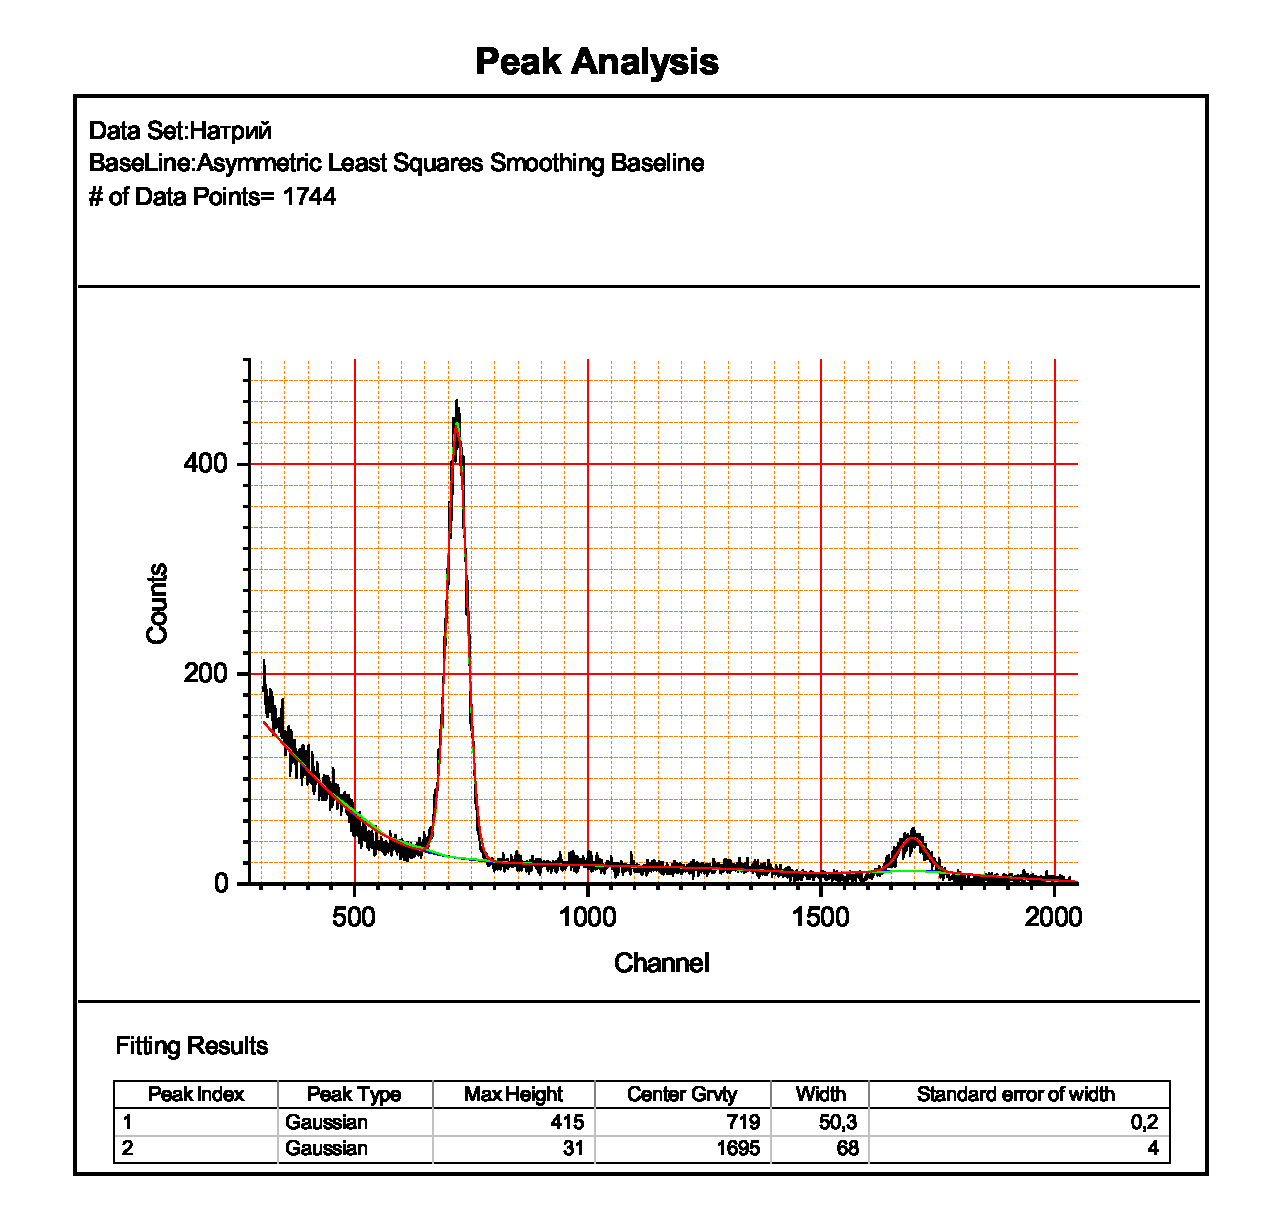
\includegraphics[width=0.8\textwidth]{1}
\caption{Энергетическое распределение, характеризующее (а) возбужденное состояние ядра (б) сдвиг линий испускания и поглощения из-за отдачи при свободных ядрах.}
\end{center}
\end{figure}

\section*{Установка}
В ходе измерения источник остаётся неподвижен, а образец поглотителя совершает равномерное движение с контролируемой скоростью. Доплеровский сдвиг изменяет частоту гамма-квантов в системе покоя поглотителя, что позволяет изучить зависимость поглощения в образце от энергии гамма-кванта. Детектируется интенсивность $\gamma$-излучения, прошедшего через образец поглотителя. При совпадении энергии гамма-кванта с разницей энергий между основным состоянием и первым возбуждённым происходит резонансное поглощения гамма-квантов и интенсивность прошедшего излучения уменьшается. Измерительная аппаратура (сцинцилятор с ФЭУ) оптимизированы под детектирование квантов с энергией 23.8 кэВ, электронная часть схемы измерения оптимизируется под обнаружение этих квантов в ходе работы. Принципиальная схема установки представлена на Рис. 2:
\begin{figure}[h!]
\begin{center}
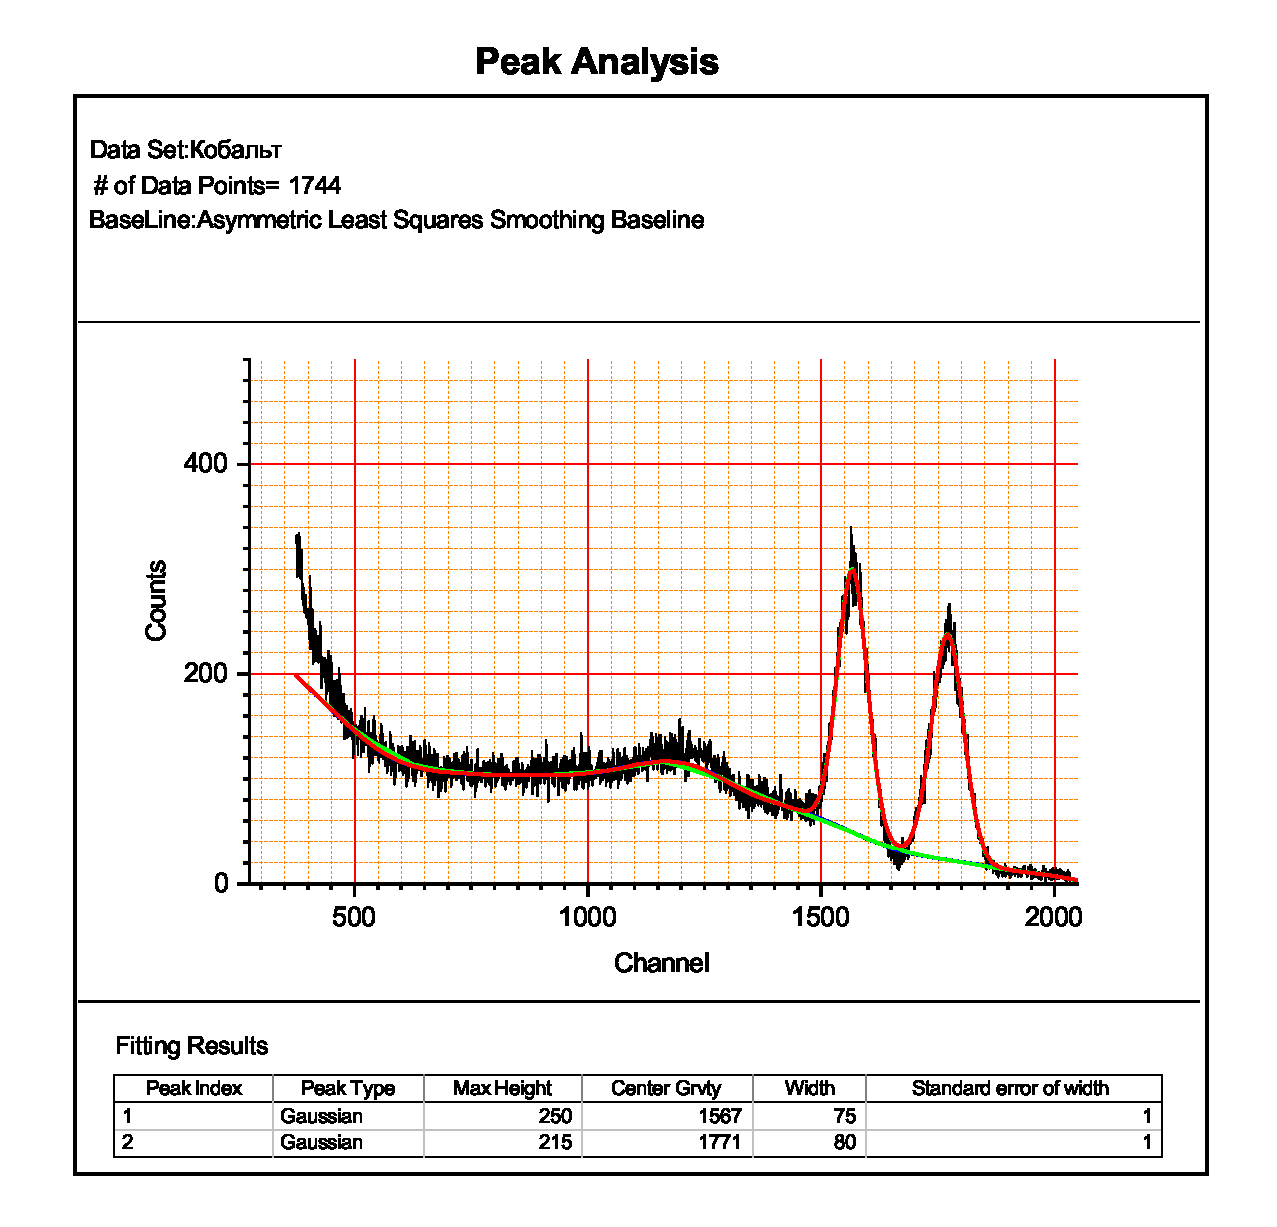
\includegraphics[width = 0.7\textwidth]{2} 
\caption{Блок-схема установки для наблюдения эффекта Мессбауэра: Э -- эксцентрик, С -- сцинтилляционный кристалл $\ce{NaI}(\ce{Tl})$, У -- усилитель, $AA$ -- одноканальный амплитудный анализатор, ЭВМ -- персональный компьютер, Г -- генератор для питания двигателя, РД-09 -- двигатель с редуктором, ВСВ -- высоковольтный стабилизированный выпрямитель}
\end{center}
\end{figure}


\section*{Выполнение и обработка данных}
Цель этого этапа работы -- подобрать настройки анализатора импульсов так, чтобы детектировались только гамма-кванты с энергией 23.8 кэВ, исходящие от источника Sn-119.

Подготовим приборы к работе. Проведём измерение спектра излучения источника при значениях нижнего порога напряжения от 0 до 9,5 В. Результаты измерения занесём в таблицу 1. Данные графически представим на Рис. 3.

\begin{table}[h!]
\begin{tabular}{|c|c|c|c|c|c|c|c|c|c|c|}
\hline
$U, $ В & 0      & 0.5   & 1     & 1.5  & 2     & 2.5   & 3     & 3.5    & 4      & 4.5    \\ \hline
$N$     & 309.4  & 141.8 & 48.4  & 86.2 & 223.6 & 500.8 & 981.8 & 1447.6 & 1665.4 & 1514.6 \\ \hline
$U, $ В & 5      & 5.5   & 6     & 6.5  & 7     & 7.5   & 8     & 8.5    & 9      & 9.5    \\ \hline
$N$     & 1022.4 & 556.4 & 246.6 & 88.4 & 33.2  & 18.4  & 10.6  & 10.6   & 9.4    & 10.8   \\ \hline
\end{tabular}
\centering
\caption{Измерение спектра источника излучения}
\end{table}

\begin{figure}[h!]
\begin{center}
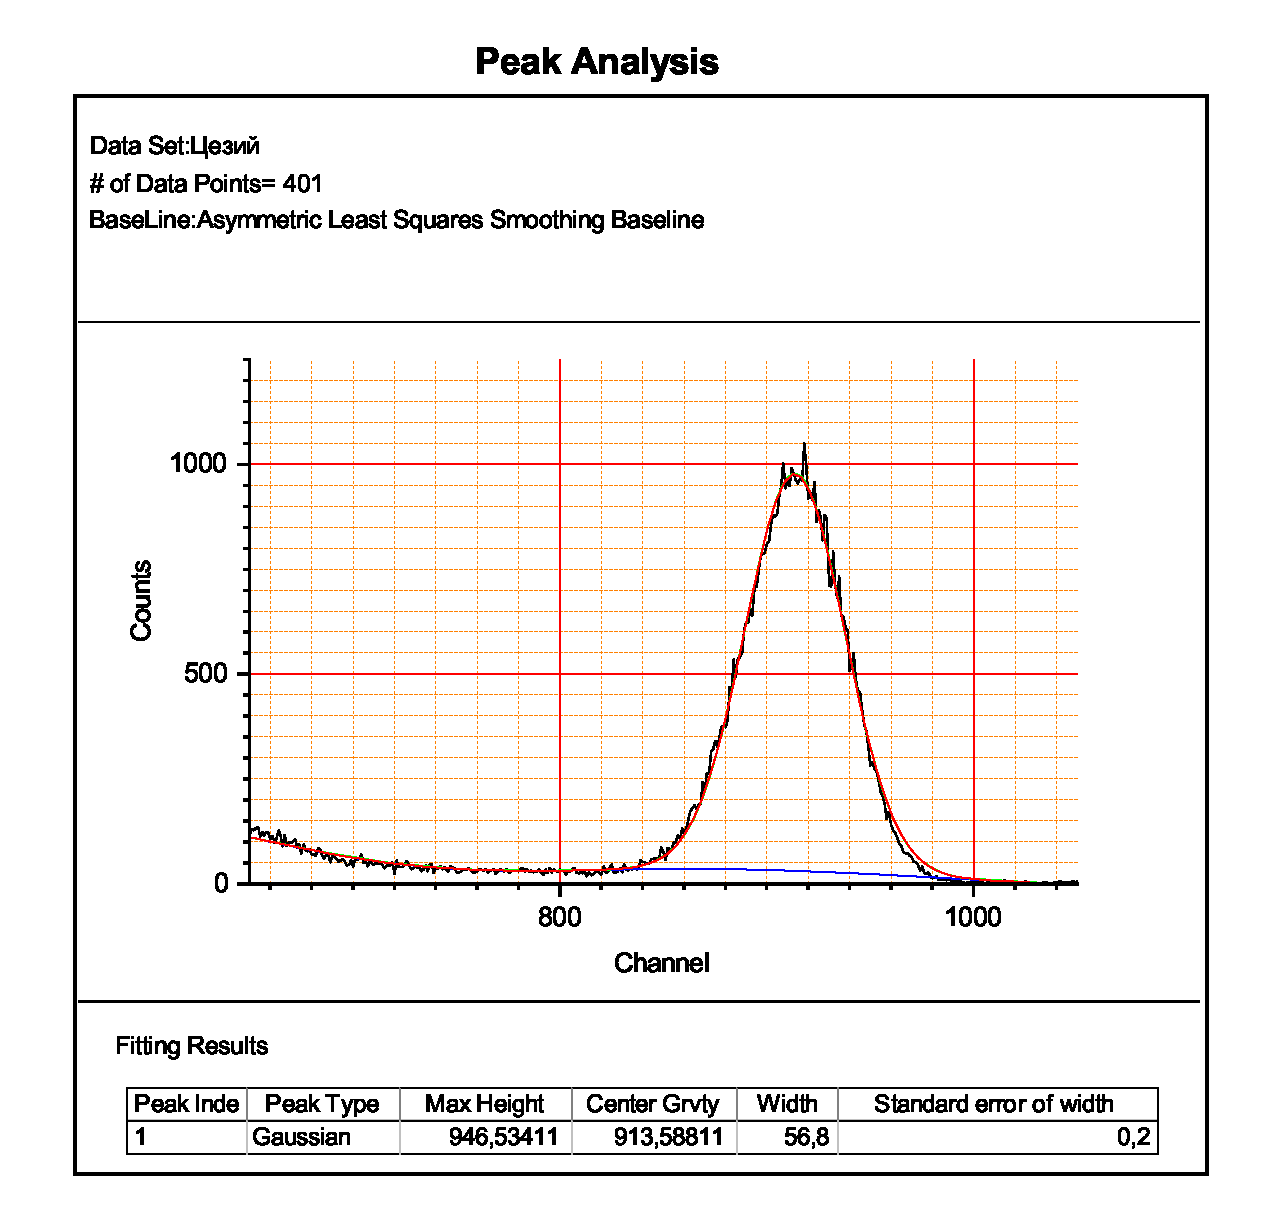
\includegraphics[width=0.7\textwidth]{3} %width = 0.7\textwidth
\caption{Спектр источника излучения}
\end{center}
\end{figure}

По графику, приведённому на рис. 3, определяем, что большая часть гамма-квантов с нужной нам энергией 23,8 кэВ появляется при пороговых значениях порядка 4 В. Установим эти значения на выпрямителе. По окончании этого этапа электронная схема нашей установки настроена так, что подсчитываются только гамма-кванты с энергиями, соответствующими используемому источнику. Теперь можно переходить к исследованию резонансного поглощения.

Измерим фоновое излучение. Вычитание фона в дальнейшем производится компьютером автоматически. Измеренное значение фона: 3,65 1/сек.

Проведём измерение спектра резонансного поглощения для четырех образцов: 3 оловянные пленки разной толщины (90 мкм, 180 мкм и 310 мкм первый, второй и третий образцы соответственно) и образец оксида олова SnO$_2$. Для этого проведём серию измерений при разных скоростях движения поглотителя. Результаты занесём в таблицы 2 и 3.



\begin{table}[h]
\begin{tabular}{|c|c|c|c|c|c|c|c|}
\hline
\multicolumn{4}{|c|}{Поглотитель   1, время измерения 30 сек} & \multicolumn{4}{c|}{Поглотитель   2, время измерения 20 сек} \\ \hline
$v-$, мм/c    & $I-$, счет    & $v+$, мм/c    & $I+$, счет    & $v-$, мм/c    & $I-$, счет    & $v+$, мм/c    & $I+$, счет   \\ \hline
0,00          & -50770        & 0,00          & 50770         & 0,00          & 31721         & 0,00          & 31721        \\ \hline
-4,59         & -35913        & 4,58          & 35748         & -4,58         & 18312         & 4,57          & 17981        \\ \hline
-4,43         & -35870        & 4,43          & 35672         & -4,41         & 18287         & 4,42          & 18015        \\ \hline
-4,25         & -35886        & 4,26          & 35503         & -4,25         & 18328         & 4,27          & 17922        \\ \hline
-4,07         & -35864        & 4,36          & 35436         & -4,07         & 18291         & 4,50          & 17917        \\ \hline
-3,89         & -35823        & 3,90          & 35342         & -3,91         & 18382         & 3,92          & 17800        \\ \hline
-3,73         & -35824        & 3,74          & 35296         & -3,72         & 18310         & 3,75          & 17641        \\ \hline
-3,54         & -35845        & 3,56          & 35218         & -3,53         & 18332         & 3,56          & 17553        \\ \hline
-3,37         & -35842        & 3,39          & 34991         & -3,35         & 18360         & 3,37          & 17338        \\ \hline
-3,16         & -35769        & 3,20          & 34793         & -3,15         & 18376         & 3,19          & 17186        \\ \hline
-2,99         & -35793        & 3,02          & 34522         & -2,98         & 18344         & 3,00          & 16969        \\ \hline
-2,79         & -35830        & 2,82          & 34167         & -2,79         & 18298         & 2,81          & 16524        \\ \hline
-2,59         & -35799        & 2,62          & 33504         & -2,58         & 18357         & 2,62          & 16174        \\ \hline
-2,39         & -35848        & 2,43          & 32928         & -2,39         & 18364         & 2,42          & 15936        \\ \hline
-2,19         & -35848        & 2,21          & 32799         & -2,19         & 18335         & 2,21          & 15831        \\ \hline
-1,97         & -35824        & 2,00          & 33347         & -1,97         & 18361         & 1,99          & 15998        \\ \hline
-1,74         & -35851        & 1,76          & 34230         & -1,73         & 18308         & 1,77          & 16742        \\ \hline
-1,48         & -35834        & 1,52          & 34923         & -1,47         & 18355         & 1,50          & 17443        \\ \hline
-1,20         & -35710        & 1,22          & 35483         & -1,19         & 18244         & 1,22          & 17909        \\ \hline
-0,77         & -35688        & 0,91          & 35640         & -0,80         & 18239         & 0,90          & 18058        \\ \hline
\end{tabular}
\caption{Поглотители 1 и 2}
\centering
\end{table}

$ $

\begin{table}[h]
\begin{tabular}{|c|c|c|c|c|c|c|c|}
\hline
\multicolumn{4}{|c|}{Поглотитель   3, время измерения 15 сек} & \multicolumn{4}{c|}{Поглотитель   4, время измерения 5 сек} \\ \hline
$v-$, мм/c    & $I-$, счет    & $v+$, мм/c    & $I+$, счет    & $v-$, мм/c    & $I-$, счет    & $v+$, мм/c   & $I+$, счет   \\ \hline
0,00          & 16378         & 0,00          & 16378         & 0,00          & 33630         & 0,00         & 33630        \\ \hline
-4,58         & 7847          & 4,61          & 7631          & -4,56         & 29810         & 4,56         & 29977        \\ \hline
-4,40         & 7831          & 4,42          & 7592          & -4,39         & 29741         & 4,39         & 29829        \\ \hline
-4,26         & 7876          & 4,25          & 7528          & -4,21         & 29760         & 4,27         & 29745        \\ \hline
-4,08         & 7875          & 4,07          & 7474          & -4,06         & 29711         & 4,05         & 29674        \\ \hline
-3,87         & 7801          & 3,90          & 7459          & -3,90         & 29774         & 3,89         & 29606        \\ \hline
-3,80         & 7804          & 3,74          & 7448          & -3,68         & 29613         & 3,74         & 29621        \\ \hline
-3,52         & 7818          & 3,55          & 7340          & -3,52         & 29402         & 3,57         & 29495        \\ \hline
-3,32         & 7870          & 3,37          & 7178          & -3,40         & 29450         & 3,38         & 29299        \\ \hline
-3,16         & 7838          & 3,19          & 7080          & -3,20         & 29436         & 3,20         & 29396        \\ \hline
-2,98         & 7802          & 3,01          & 6958          & -3,00         & 29270         & 2,97         & 29225        \\ \hline
-2,80         & 7789          & 2,80          & 6772          & -2,76         & 29029         & 2,78         & 29083        \\ \hline
-2,59         & 7822          & 2,61          & 6515          & -2,61         & 29062         & 2,61         & 28911        \\ \hline
-2,38         & 7808          & 2,40          & 6340          & -2,38         & 28770         & 2,42         & 28844        \\ \hline
-2,18         & 7833          & 2,20          & 6342          & -2,17         & 28586         & 2,20         & 28542        \\ \hline
-1,98         & 7827          & 2,00          & 6484          & -1,97         & 28162         & 1,99         & 28300        \\ \hline
-1,72         & 7866          & 1,76          & 6889          & -1,75         & 27788         & 1,78         & 27920        \\ \hline
-1,46         & 7826          & 1,49          & 7275          & -1,48         & 26994         & 1,50         & 27160        \\ \hline
-1,20         & 7817          & 1,22          & 7515          & -1,21         & 26045         & 1,25         & 26394        \\ \hline
-0,82         & 7803          & 1,33          & 7647          & -0,84         & 23878         & 1,85         & 24718        \\ \hline
\end{tabular}
\centering
\caption{Поглотители 3 и 4}
\end{table}

По результатам измерения построим графики спектров резонансного поглощения для разных поглотителей (рис. 4-7). По графикам определим амплитуду резонансного поглощения в максимуме (в процентах) для образцов 1-3, величину химического сдвига (в мм/с и в эВ) и экспериментальную ширину линии $\Gamma$. К сожалению, для образца оксида олова соответствующие измерения сделать не удалось, поскольку не удалось промерить околонулевые скорости.

\begin{figure}[h!]
\begin{center}
\includegraphics[width=0.7\textwidth]{4} 
\caption{Поглотитель 1}
\end{center}
\end{figure}

\begin{figure}[h!]
\begin{center}
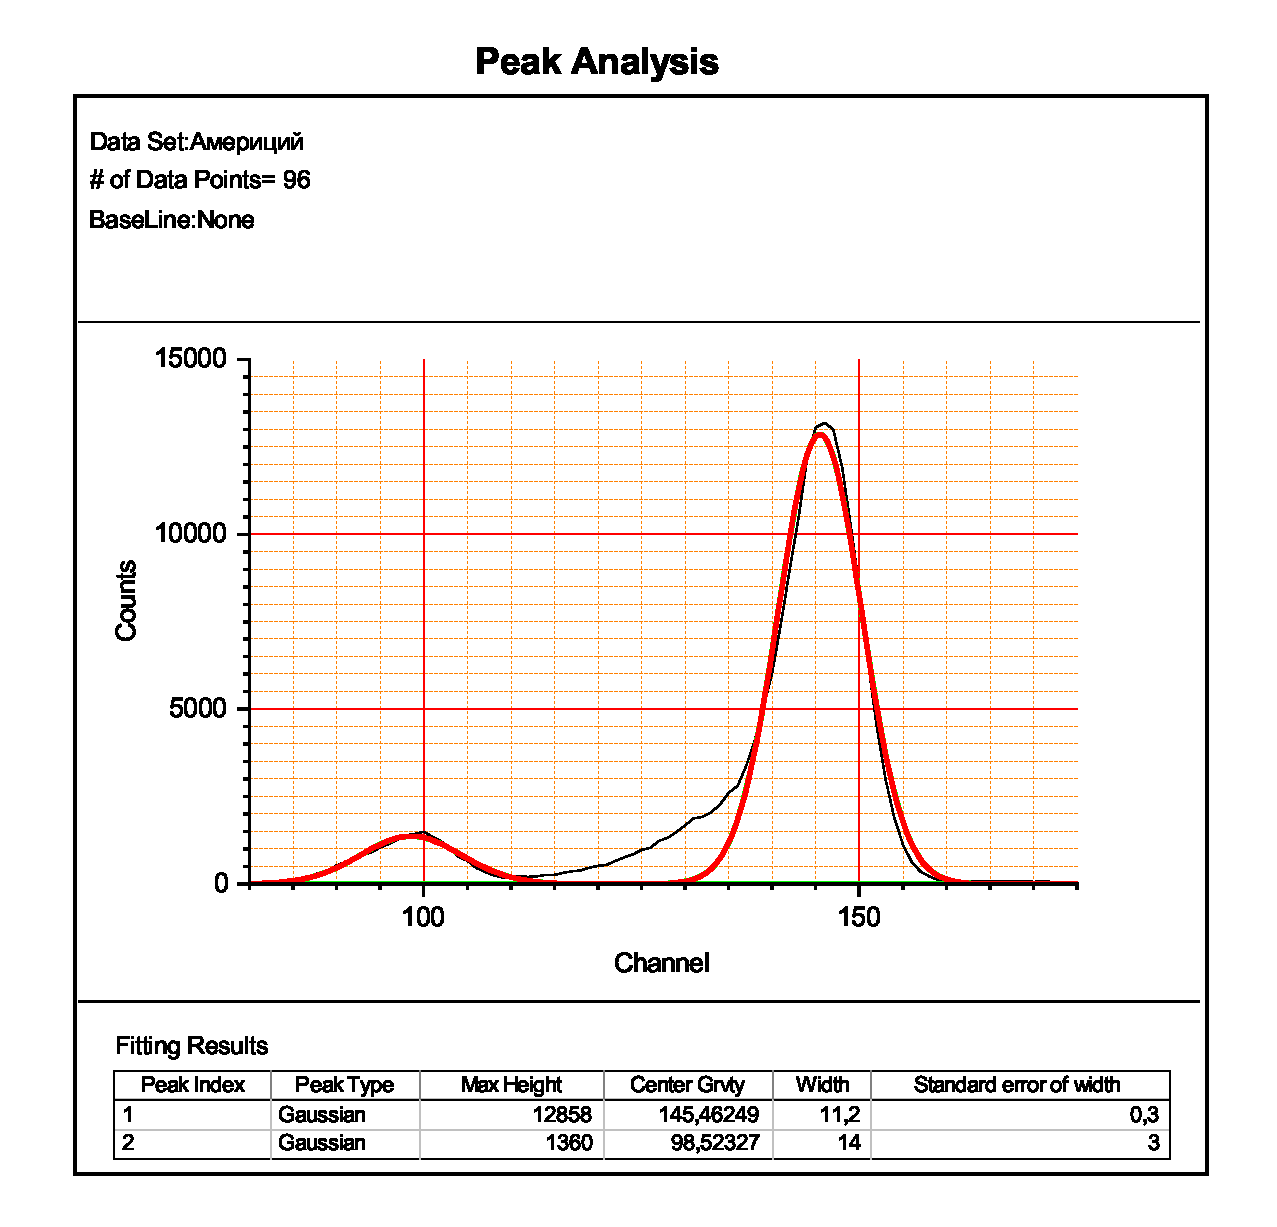
\includegraphics[width=0.7\textwidth]{5} 
\caption{Поглотитель 2}
\end{center}
\end{figure}

\begin{figure}[h!]
\begin{center}
\includegraphics[width=0.7\textwidth]{6} 
\caption{Поглотитель 3}
\end{center}
\end{figure}

\begin{figure}[h!]
\begin{center}
\includegraphics[width=0.7\textwidth]{7} 
\caption{Поглотитель 4}
\end{center}
\end{figure}

\newpage
$ $
\newpage
$ $
Формула для вычисления величины амплитуды эффекта Мессбауэра:
$$
\varepsilon(v) = \frac{N(\infty) - N(v)}{N(\infty) - N_\text{ф}},
$$
где $N(\infty)$ -- скорость счёта квантов при достаточно большой скорости, $N(v)$ -- скорость счёта квантов, прошедших через поглотитель при некоторой скорости, $N_\text{ф}$ -- скорость счёта радиоактивного фона (вычитается программой автоматически).

Величина химического сдвига, выраженная в эВ:
$$
\Delta E = E \frac{v}{c},
$$
где $E$ -- энергия гамма-кванта, излучаемого веществом (в нашем случае $E$ = 23.8 кэВ).

Экспериментальная ширина линии Г$_e$, выраженная в эВ:

$$
\Gamma_e = 2 \Gamma = E \frac{v_\Gamma}{c}.
$$

\begin{table}[h!]
\begin{tabular}{|c|c|c|c|c|c|}
\hline
              & Ампл. эффекта, \% & Хим. сдвиг, мм/с & Хим. сдвиг, $10^{-7}$ эВ & Г$_e$, мм/с & Г$_e$, $10^{-7}$ эВ \\ \hline
Погл. 1 &      3,92                 &   2,20               &      1,75          &      1,5       &     1,19      \\ \hline
Погл. 2 &      5,52                 &   2,25               &      1,79          &      1,6       &     1,27      \\ \hline
Погл. 3 &      8,44                 &   2,27               &      1,80          &      1,6       &     1,27      \\ \hline
\end{tabular}
\end{table}

\section*{Обсуждение}
В ходе работы с помощью метода доплеровского сдвига для нескольких образцов поглотителя Sn были определены амплитуда резонансного поглощения, химический сдвиг и экспериментальное значение ширины спектральной линии. Было оценено время жизни мессбауэровского ядерного уровня 23,8 кэВ: по порядку величины оно совпало с табличным значением.

\begin{thebibliography}{9}
\bibitem{laba} 
Игошин Ф.Ф., Самарский Ю.А., Ципенюк Ю.М.
\textit{Лабораторный практикум по общей физики: Учеб. пособие для вузов. Т3. Квантовая физика.}. 
М.: Физматкнига - 2005.
\end{thebibliography}
\end{document}










